\chapter{量子光通信的理论基础}

\section{电磁场的量子态描述}
\subsection{相干态}
通信中常用相干光来传递信息,它可以用一个正弦波来表示。
不失一般性,可以用线偏振的电场来实现\cite{djordjevic2010fundamentals},
\begin{equation}
\bm{E}(t) = \bm{p} A e^{j\omega t + \phi}.
\end{equation}
上式中,符号$\bm{p}$、$A$、$\omega$和$\phi$分别对应偏振矢量、幅度、频率和相位。
要传递的信息被调制在场的这四个要素上面。
在本文中,主要关注的是对幅度和相位的调制。
这两个要素可以用一个复振幅来描述
\begin{equation}
\alpha = A e^{j\phi}.
\end{equation}
也可以用相空间复平面中的一个点来表示该复振幅,这种图像称作星座图。
图\ref{fig:signals}展示了OOK、BPSK、QPSK、16-QAM四种常见的调制信号的星座图。

\begin{figure}
\centering
  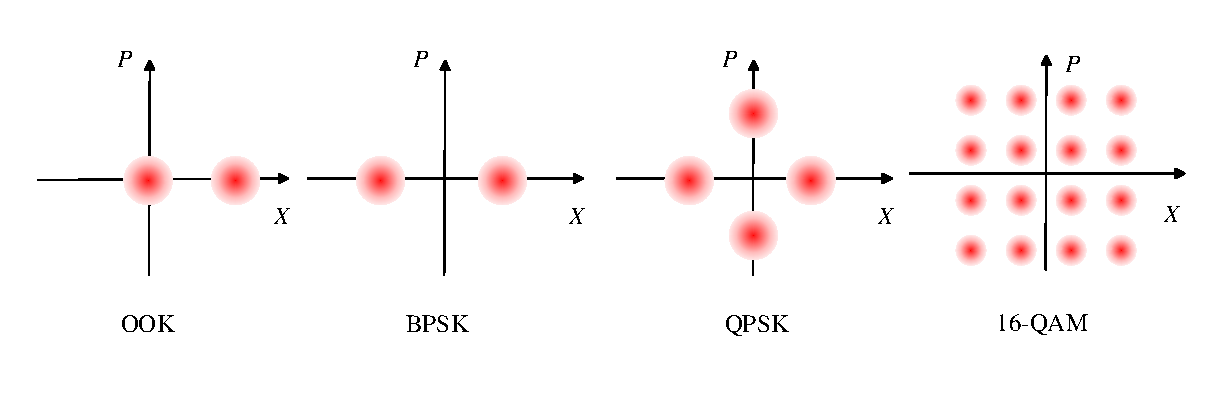
\includegraphics[width=\textwidth]{figures/chap2/signals}
  \caption{常见的四种调制信号星座图}
  \label{fig:signals}
\end{figure}

在量子力学中,电磁场被量子化为若干个不同模式、不同频率的光子\cite{gerry2005introductory,helstrom1976quantum,mandel1995optical}。
单模电磁场的哈密顿量可以表示为
\begin{equation}
\hat{H} = \hbar \omega (\hat{a}^\dagger \hat{a} + \frac{1}{2}).
\end{equation}
其中$\hat{a}^\dagger$和 $\hat{a}$ 分别是产生算符和湮灭算符,
乘积$\hat{a}^\dagger \hat{a}$是粒子数算符,他的本振态是Fork态$\ket{n}$。
\begin{equation}
\hat{a}^\dagger \hat{a} \ket{n} = n \ket{n}.
\end{equation}

通信中常用的单模相干光脉冲可以用单模相干态$\ket{\alpha}$来描述,它是湮灭算符的本振态
\begin{equation}
\hat{a} \ket{\alpha} = \alpha \ket{\alpha}.
\end{equation}
在Fork态表象中,相干态可以表达为
\begin{equation}
\ket{\alpha} = \exp(-\frac{1}{2}|\alpha|^2) \sum_{n=0}^\infty \frac{\alpha^n}{\sqrt{n!}} \ket{n}.
\end{equation}
如果用光子计数器进行探测,相干态$\ket{\alpha}$探测到的光子数不是一个固定的值,
而是服从泊松分布
\begin{equation}
P_n = |\bra{n}\ket{\alpha}|^2 = \exp(-|\alpha|^2) \frac{|\alpha|^{2n}}{n!} .
\end{equation}
它的平均光子数由
\begin{equation}
\bar{n} = |\alpha|^2
\end{equation}
给出。相干态参数${\alpha}$可以是任何复数,具有复振幅的意义\cite{glauber1963coherent}。

数学上也常常用密度矩阵来表示信号\cite{wt2001qm},相干态$\ket{\alpha}$也可以用密度矩阵表示为
$\ket{\alpha}\bra{\alpha}$。



\subsection{位移操作}

\begin{figure}
\centering
  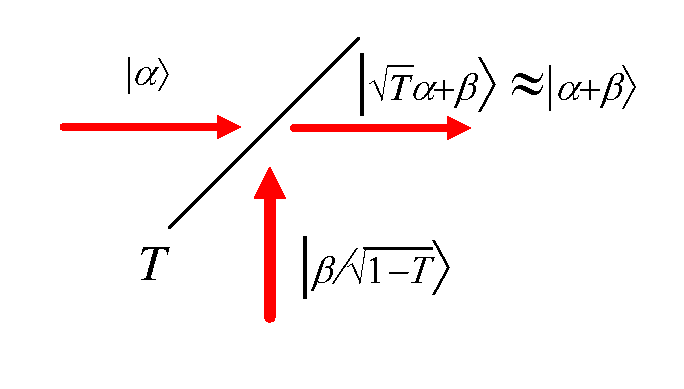
\includegraphics[height=5cm]{figures/chap2/displacement-operator}
  \caption{用波束分束器实现位移操作示意图}
  \label{fig:diaplacement}
\end{figure}

相干态可以通过位移操作进行变换,位移算符定义为\cite{glauber1963coherent,gerry2005introductory,helstrom1976quantum,mandel1995optical}
\begin{equation}
\hat{D}(\alpha) = \exp(\alpha \hat{a}^\dagger - \alpha^* \hat{a}).
\end{equation}
利用位移算符,相干态可以通过对真空态$\ket{0}$位移得到
\begin{equation}
\hat{\alpha} = \hat{D}(\alpha) \ket{0}.
\end{equation}
两个相干态之间也可以通过位移操作进行转换
\begin{equation}
\hat{D}(\beta) \ket{\alpha} = \ket{\alpha + \beta} .
\end{equation}


在实验当中,常用一个相位稳定干涉仪或者波束分束器来实现\cite{cook2007optical,becerra2013experimental,lau2006binary,paris1996displacement}。
图\ref{fig:diaplacement}显示的是利用一个高透过率的波束分束器,
将两个入射场混合输出,近似实现了对其中一个入射场的位移操作。
这种方案在量子接收机实验中经常见到。

\section{经典光通信的接收方案}

\subsection{引言}
在经典光通信中,有三类常见的接收方案,他们分别是
直接检测、零差接收和外差接收。
这三种接收方案受散粒噪声的制约,
使得每一种接收方案存在一个经典极限
——标准量子极限(Standard Quantum Limit)。
接下来,我们简单介绍一下每一种接收方案的具体实现方案。

\subsection{直接检测}

在所有的调制方案中,有一类采用脉冲的有无对信息进行编码,
比如开关键控(OOK)和脉冲位置调制(PPM)。
OOK调制将符号0编码为没有光脉冲,
而将符号1编码为有脉冲;PPM调制则将信息编码到脉冲所在的位置上。
对于这样一类的调制方案,经典光通信中常采用直接检测方案进行探测。
如图\ref{fig:DD}所示,直接检测方案直接探测信号光的强度,
来判断是否存在光脉冲或者光脉冲的幅度\cite{gagliardi1976optical,gagliardi1998optical}。
这种方案可以利用一个光电探测器或单光子探测器实现。
探测器可以输出探测到的光子数目,理想情况下,
对于给定的相干态,探测到$n$个光子的概率
\begin{equation}
\Pr(N = n| \ket{\alpha}) = \frac{|\alpha|^{2n}}{n!} e^{-|\alpha|^2}
\label{eq:dd-prob}
\end{equation}
一般地,对于信号矢态为$\ket{\phi}$的情况下,检测概率为
\begin{equation}
\Pr(N = n| \ket{\phi}) = |\bra{n}\ket{\phi}|^2
\end{equation}



\begin{figure}
\centering
  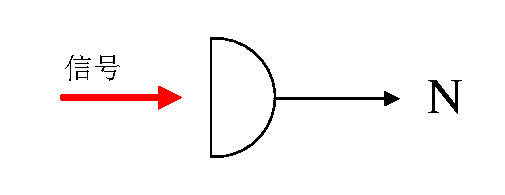
\includegraphics[scale=1]{figures/chap2/DD.pdf}
  \caption{直接检测示意图}
  \label{fig:DD}
\end{figure}


\subsection{零差接收}
零差接收机是一种相干检测方案,如图\ref{fig:HD}所示,
是一种平衡零差接收方案\cite{gagliardi1976optical,gagliardi1998optical}。
这种接收方案和直接检测不同的是,
需要一个本振。对于零差接收本振频率和信号频率一致。
通常本振强度$a_{LO}$远大于信号强度$a_S$,
两路信号通过一个50:50的分束器,
在两个输出口得到两路新的信号$a_+$和$a_-$,满足关系式
\begin{equation}
a_\pm = \frac{a_S \pm a_{LO}}{\sqrt{2}}.
\end{equation}
这两路信号被光电探测器接收,得到两路光电流$i_\pm$。
这两路电流通过一个放大系数为$\frac{1}{K}=\frac{1}{2q\sqrt{N_{LO}}}$的差分放大器,
最后通过一个低通滤波器积分得到输出统计量
\begin{equation}
\alpha_\theta = \frac{N_+ - N_-}{2\sqrt{N_{LO}}}.
\end{equation}
这里假定所有的器件都是理想的。当$N_{LO} \rightarrow \infty$时,
输出统计量服从高斯分布
\begin{equation}
\alpha_\theta \sim N(Re(ae^{-j\theta}), \frac{1}{4}).
\end{equation}
其中$\theta$是本振与信号的相位差。
这种测量方案,用量子力学算符可以用湮灭算符描述为\cite{yuen1980optical,mandel1995optical}
\begin{equation}
\hat{\alpha}_\theta = \Re(\hat{a}_S e^{-j\theta}).
\end{equation}


\begin{figure}
\centering
  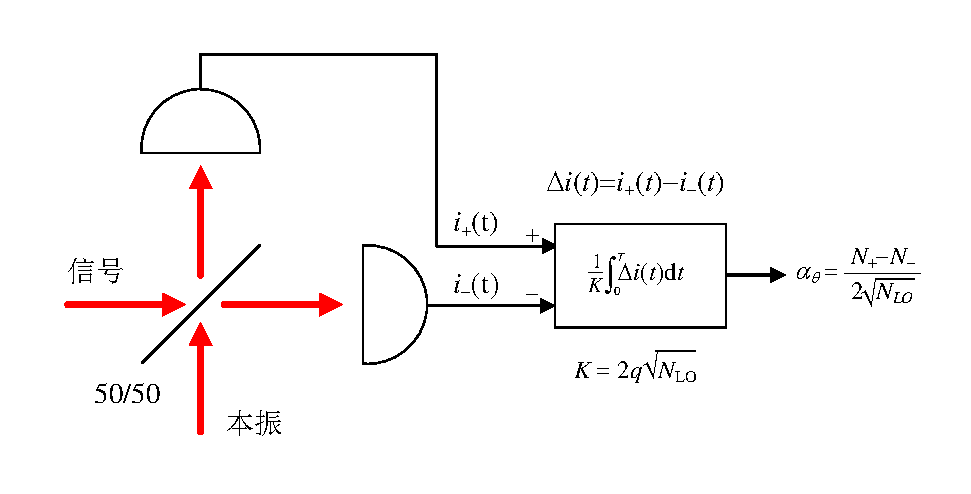
\includegraphics[width=0.8\textwidth]{figures/chap2/homodyne-receiver.pdf}
  \caption{平衡零差检测示意图}
  \label{fig:HD}
\end{figure}

\subsection{外差接收}
在上一小节,我们已经介绍了零差接收方案。
另外一种相干接收方案是外差接收\cite{gagliardi1976optical,gagliardi1998optical},
它采用了与信号频率不同的本振。
图\ref{fig:HeD}是一种平衡外差接收机示意图,
在这种外差接收机中,频率为$\omega$的信号场$a_S$
与频率为$\omega - \omega_{IF}$的强本振场$a_{LO}$
通过一个50:50的分束器混合。
混合后经过光电探测器,得到两路以中频$\omega_{IF}$震荡的电流$i_\pm$。
这两路电流经过一个放大系数为$\frac{1}{K'}=\frac{1}{q\sqrt{N_{LO}}}$的差分放大器,
最后解调出两个正交幅度$\alpha_1$和$\alpha_2$。
假定所有的器件都是理想的,当$N_{LO} \rightarrow \infty$时,
这两个统计量统计独立,分别服从高斯分布
\begin{equation}
\alpha_i \sim N(a_{S_i}, \frac{1}{2}).
\end{equation}
其中$a_{S_1}=\Re(a_S)$和$a_{S_2}=\Im(a_S)$分别是信号场的两个正交幅度。
这种测量方案,用量子力学算符湮灭算符可以描述为\cite{yuen1980optical,mandel1995optical}
\begin{equation}
\hat{\alpha}_1 + j \hat{\alpha}_2 = \hat{a}_S.
\end{equation}



\begin{figure}
\centering
  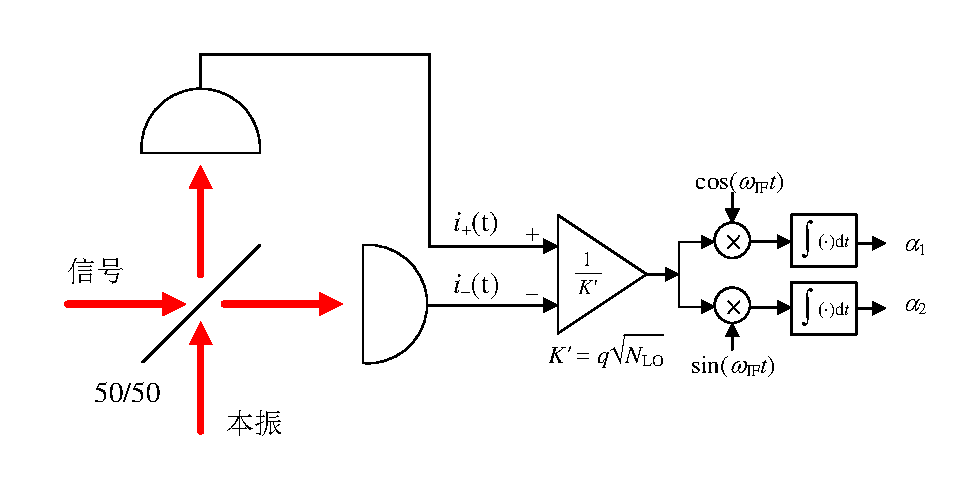
\includegraphics[width=0.8\textwidth]{figures/chap2/heretrodyne-receiver.pdf}
  \caption{平衡外差检测示意图}
  \label{fig:HeD}
\end{figure}


\section{量子检测与估计理论}
\subsection{经典最优检测}
通信系统通常由发送端、信道和接收端三个部分组成。
对某种特定的通信方案,发送端通常从$M$个符号中选择一个发送出去。
我们称一个假设$H_j (j=1,2,...,M)$是指发送的是第$j$个符号。
对于这$M$个符号,我们赋予它们一个先验概率$\zeta_j$,
先验概率满足归一化条件
\begin{equation}
\sum_{j=1}^M \zeta_j = 1.
\end{equation}


在通信的接收端,接收机对电磁场进行探测,可以得到一些统计量。
例如在前面介绍的三种经典监测方案,输出的统计量分别是光子数目、
$\alpha_\theta$、$\{\alpha_1, \alpha_2\}$。
由于量子涨落或者噪声的影响,对于给定的发送信号,
这些统计量通常不是一个固定的值,而是一个随机变量。
一般的,我们假设输出统计量是一个随即向量$\bm{v} = (v_1, v_2, ..., v_n)$。
当发送第$j$个符号时,
假定它的联合分布为
$p_j(\bm{v}) = p_j(v_1, v_2, ..., v_n)$。
在通信的接收端,通过对接收到的统计量进行判决,
判定发送的符号是哪一个。
下面介绍两种重要的准则——贝叶斯准则和最小错误概率准则。

我们定义决策代价$C_{ij}$为,
当假设$H_j$是正确的情况下,选择了假设$H_i$所需要的代价。
我们期望一个决策是最优的是指该决策所需要的代价最小。

我们再来将决策数学化\cite{yzf2002tjxhcl,helstrom1976quantum},
定义在观测到的统计量为$\bm{v}$时,
选择了假设$H_i$的概率为$\pi_i(\bm{v})$,$i=1,2,...,M$。
这些决策概率需满足条件
\begin{equation}
0 \le \pi_i(\bm{v}) \le 1,  \sum_{i=1}^M \pi_i(\bm{v}) = 1.
\label{eq:pi-cond}
\end{equation}
一个简单的例子是一种被称为随机策略的决策方案,
对于任意观测量,这种策略都是随机选择一个假设,
即$\pi_i(\bm{v}) \equiv 1/M, \forall i, \bm{v}$。

在上述符号的约定下,我们可以得到在假设$H_j$是正确的情况下,
策略选择了假设$H_i$的条件概率为
\begin{equation}
\Pr\{i|j\} = \int_R \pi_i(\bm{v}) p_j(\bm{v}) d^n \bm{v}.
\end{equation}
那么,对所有的观测结果,平均代价为
\begin{equation}
\begin{split}
\bar{C} &= \sum_{i=1}^M \sum_{j=1}^M \zeta_j C_{ij} \Pr{i|j} \\
 &= \sum_{i=1}^M \sum_{j=1}^M \zeta_j C_{ij} \int_R \pi_i(\bm{v}) p_j(\bm{v}) d^n \bm{v}.
\end{split}
\end{equation}
对于每一个假设$H_i$,我们定义它的风险函数
\begin{equation}
W_i(\bm{v}) = \sum_{j=1}^M \zeta_j C_{ij} p_j(\bm{v})。
\end{equation}
那么决策的平均代价可以改写为
\begin{equation}
\bar{C} =  \int_R \sum_{i=1}^M W_i(\bm{v}) \pi_i(\bm{v}) d^n \bm{v}.
\label{eq:avg-C}
\end{equation}

在式\ref{eq:pi-cond}条件下,最小化式\ref{eq:avg-C},
这是一个凸优化问题。
这个问题可以通过一个简单的观察得以解决。
从式\ref{eq:pi-cond}和\ref{eq:avg-C}可以看出,
对于每一个观测结果$\bm{v} \in R$,要使得平均代价最小,
需要选择风险$W_i(\bm{v})$最小的那一个假设。
即对于每一个观测结果$\bm{v} \in R$,若
\begin{equation}
W_j(\bm{v}) < W_i(\bm{v}), \forall i \neq j,
\end{equation}
那么
\begin{equation}
\pi_j(\bm{v})=1, \pi_i(\bm{v}) \equiv 0, \forall i \neq j.
\end{equation}

为方便记函数
\begin{equation}
\Upsilon(\bm{v}) = \min_j W_j(\bm{v}), 
\end{equation}
那么对所有的观测结果$\bm{v}$和所有的假设$H_i$,有下式成立
\begin{equation}
\begin{split}
[W_i(\bm{v}) - \Upsilon(\bm{v})] \pi_i(\bm{v}) &= 0,  \\
W_i(\bm{v}) - \Upsilon(\bm{v}) &\ge 0.
\label{eq:classic-opt-cond}
\end{split}
\end{equation}
对式\ref{eq:classic-opt-cond}的第一个式子求和,可以得到
\begin{equation}
\Upsilon(\bm{v}) = \sum_i^M W_i(\bm{v})\pi_i(\bm{v}), 
\end{equation}
因此,可以得到最小平均代价为
\begin{equation}
\bar{C}_{min} = \int_R \Upsilon(\bm{v}) d^n \bm{v}. 
\end{equation}
容易验证,这样得到的平均代价确实是最小平均代价,
即对任意其他的决策函数$\{\pi_i'(\bm{v})\}$,有
\begin{equation}
\bar{C}' - \bar{C}_{min} = \sum_{i=1}^M \int_R [W_i(\bm{v}) - \Upsilon] \pi_i'(\bm{v}) d^n \bm{v} \ge 0. 
\end{equation}


现代的文献中,常将这种最小化平均代价函数的决策称作贝叶斯准则。
在这当中,有一种被称为最小错误概率准则的策略,它的决策代价系数定义为
\begin{equation}
C_{ii} = -1; C_{ij}=0, \forall i\neq j. 
\label{eq:min-err-cond}
\end{equation}
在这种决策代价下,最小平均代价就是最小平均错误概率
\begin{equation}
P_e = 1 - \sum_{j=1}^M \zeta_j \Pr{j|j} = \sum_{j=1}^M \zeta_j \sum_{k\neq j}\Pr{k|j}.
\end{equation}
在通信中,常用最小平均错误概率准则来设计接收机的接收策略。
因此本文也主要以该准则来设计量子接收机。

通过经典的三种探测方式加上经典检测预估计理论所得到的最佳接收方案,
它能达到的最小平均错误概率通常被称作标准量子极限(SQL)。




\subsection{量子最优检测}
上世纪六十年代,C.W. Helstrom和H. P. Yuen等人
将假设检验理论与量子力学结合起来,
发展出一套适用于量子测量的量子检测与估计理论
\cite{helstrom1976quantum,helstrom1967detection,yuen1975optimum}。
根据这一套理论,可以从理论上给出最优检测的数学形式,
下面我们简单回顾一下这个理论的主要内容。

在量子力学中,一个测量在数学上被描述为一个正定算子值测量(POVM)算符\cite{helstrom1976quantum}。
如果用算符$\hat{\Pi}_i (i=1,2,...,M)$表示一组POVM测量,
那么一组完备的POVM测量需要满足条件
\begin{equation}
\begin{split}
\hat{\Pi}_i & \ge 0, \\
\sum_{i=1}^M \hat{\Pi}_i & = \hat{I}.
\end{split}
\end{equation}

例如,直接检测利用POVM算符可以表达为
\begin{equation}
\hat{\Pi}_n = \ket{n}\bra{n}, n=0,1,2,...
\end{equation}
其中$\ket{n}$是Fork态矢量,这是一组正交投影测量。
我们说一组测量是正交投影测量是指它们满足正交条件
\begin{equation}
\hat{\Pi}_i \hat{\Pi}_j = 0, \forall i \neq j
\end{equation}
和投影算符条件
\begin{equation}
\hat{\Pi}_n^2 = \hat{\Pi}_n, n=0,1,2,...
\end{equation}
如果直接检测采用On-Off探测器,即只能探测到有光子还是没有光子,
那么直接检测对应于一个二元测量
\begin{equation}
\hat{\Pi}_0 = \ket{0}\bra{0}, \hat{\Pi}_1 = \hat{I} - \ket{0}\bra{0}.
\end{equation}


假设发送的信号态用密度矩阵为$\hat{\rho}_j$,那么将符号$j$检测为符号$i$的条件概率为
\begin{equation}
\Pr(i|j) = \Tr(\hat{\rho}_j \hat{\Pi}_i), (i,j)=1,2,...,M.
\end{equation}
那么利用上一节的符号定义,在这样的信号和测量设置下,
总的平均代价为
\begin{equation}
\bar{C} =  \sum_{i=1}^M \sum_{j=1}^M \zeta_jC_{ij} \Tr(\hat{\rho}_j \hat{\Pi}_i) \\
        =  \Tr \sum_{i=1}^M \hat{W}_i \hat{\Pi}_i.
\label{eq:q-avg-C}
\end{equation}
这里,风险算符$\hat{W}_i$定义为
\begin{equation}
\hat{W}_i = \sum_{j=1}^M \zeta_jC_{ij}\hat{\rho}_j.
\end{equation}
这样,我们得到与经典检测理论对应的优化问题。
H. P. Yuen和C. W. Helstrom等人给出该优化问题的一个充要条件,
\begin{equation}
\begin{split}
(\hat{W}_i - \hat{\Upsilon})\hat{\Pi}_i = \hat{\Pi}_i(\hat{W}_i - \hat{\Upsilon}) & = \bm{0}, i=1,2,...,M,  \\
\hat{W}_i - \hat{\Upsilon} & \ge \bm{0}, i=1,2,...,M.
\label{eq:optim-povm-cond}
\end{split}
\end{equation}
其中拉格朗日算符
\begin{equation}
\hat{\Upsilon} = \sum_{j=1}^M \hat{\Pi}_j\hat{W}_j = \sum_{j=1}^M\hat{W}_j\hat{\Pi}_j.
\end{equation}
那么,最小平均代价可以简化为
\begin{equation}
\bar{C}_{min} = \Tr(\hat{\Upsilon}).
\end{equation}

若取式\ref{eq:min-err-cond}中的最小平均错误概率准则决策代价系数,
那么最优检测问题可以简化为
\begin{equation}
\begin{split}
\max_{\hat{\Pi}_i}  \quad  &  \sum_{i=1}^M \Tr(\hat{\rho}_i'\hat{\Pi}_i) \\
s.t. \quad  & \hat{\Pi}_i \ge 0, i=1,2,...,M   \\
     \quad  & \sum_{i=1}^M \hat{\Pi}_i = \hat{I}.
\end{split}
\end{equation}
上式中,$\hat{\rho}_i' = \zeta_i \hat{\rho}_i$。
该问题是一个半正定规划(SDP)问题,
需要求解的未知矩阵个数是$M$,
可以通过求解其对偶问题将问题简化
为未知矩阵只有1个的半正定规划问题\cite{eldar2003designing}
\begin{equation}
\begin{split}
\min_{\hat{X}}  \quad & \Tr(\hat{X}) \\
s.t.          \quad & \hat{X} \ge \hat{\rho}_i', i=1,2,...,M.
\end{split}
\end{equation}
利用一种为Matlab编写的凸优化工具箱CVX,
可以很方便地求解上述半正定规划问题\cite{cvx,gb08}。

利用量子检测预估计理论计算出来的最小错误概率,
通常称作这种信号的Helstrom极限,
通常比经典检测方案所能达到的极限要低很多\cite{helstrom1976quantum}。



\subsection{平方根检测}
一般情况下,为了求解量子最优测量问题,
需要利用数值优化工具进行数值计算,
只有很少数情况下可以得到解析表达式。
因此,这不利于理论研究。
而平方根检测是一种解析方法,通过信号矢量的Gram矩阵的平方根
构造出来的一组POVM算符进行测量\cite{hausladen1994pretty,hausladen1996classical}。
在最小错率概率准则下,它是一种近最优的检测方案,
但是在最小均方误差准则下,它是最优的。
并且,在信号具有几何均匀对称性的情况下,
它也是最小错误概率准则下的最优检测\cite{kato1999quantum,eldar2001quantum,cariolaro2010performance,cariolaro2010theory}。
在很多理论问题的研究中,由于平方根检测具有良好的解析表达式,
常常被用来作为一种理论检测方案进行研究\cite{hausladen1996classical,sasaki1998quantum,guha2012polar}。
下面,我们介绍一下这种接收方案的数学形式。

设$M$个信号由$n$维Hilbert空间$\mathcal{H}$中
的向量表示为$\ket{\psi_i}(i=1,2,...M)$,对应的密度矩阵为
$\hat{\rho}_i = \ket{\psi_i} \bra{\psi_i}$。
这些信号张成$\mathcal{H}$中一个$r\le M$维子空间$\mathcal{U}$。
当且仅当$M$个信号线性独立时,等号成立$r=M$。
$M$个POVM测量满足
\begin{equation}
\hat{\Pi}_i \ge 0, \sum_{i=1}^M \hat{\Pi}_i = \hat{I}_r.
\end{equation}
这里$\hat{I}_r$是子空间$\mathcal{U}$上的单位矩阵。

将信号的密度矩阵和POVM测量矩阵分解为
\begin{equation}
\begin{split}
\hat{\rho}_i & = \hat{\gamma}_i \hat{\gamma}_i^\dagger,\\
\hat{\Pi}_i & = \hat{\mu}_i \hat{\mu}_i^\dagger.
\end{split}
\end{equation}
重新定义信号集合矩阵$\hat{\Gamma}=[\hat{\gamma}_1 \quad \hat{\gamma}_2 \quad ...\quad \hat{\gamma}_M]$
和POVM测量集合矩阵$\hat{M} = [\hat{\mu}_1\quad \hat{\mu}_2\quad ...\quad \hat{\mu}_M]$。
Gram矩阵定义为$\hat{T} = \hat{\Gamma} \hat{\Gamma}^\dagger$
和$\hat{G} = \hat{\Gamma}^\dagger \hat{\Gamma}$,
平方根检测给出的POVM测量集合矩阵为
\begin{equation}
\hat{M} = \hat{T}^{-\frac{1}{2}} \hat{\Gamma} = \hat{\Gamma} \hat{G}^{-\frac{1}{2}}.
\end{equation}
可以证明这种POVM测量使得均方误差
\begin{equation}
E = \Tr[(\hat{\Gamma} - \hat{M})^\dagger (\hat{\Gamma} - \hat{M})]
\end{equation}
达到最小值\cite{eldar2001quantum}。

在平方根检测的POVM测量算符下,
将信号$i$判断为$j$的条件概率为
\begin{equation}
\begin{split}
\Pr{j|i} = \Tr(\hat{\rho}_i \hat{\Pi}_j) & = \Tr(\hat{\gamma}_i \hat{\gamma}_i^\dagger \hat{\mu}_j \hat{\mu}_j^\dagger) \\
     =\Tr(\hat{\mu}_j^\dagger\hat{\gamma}_i \hat{\gamma}_i^\dagger \hat{\mu}_j )     & = \Tr(\hat{B}_{ji} \hat{B}_{ji}^\dagger).
\end{split}
\end{equation}
这里矩阵$\hat{B}_{ji}$是矩阵 $\hat{M}^\dagger \hat{\Gamma} = \hat{G}^{1/2}$的第$(j,i)$子块$\hat{\mu}_j^\dagger\hat{\gamma}_i$。
对于纯态信号集合,信号密度矩阵秩为1,因此$\hat{\gamma}_i$和$\hat{\mu}_i$是一个向量,
因此
\begin{equation}
\Pr{j|i} = (\hat{G}^{1/2})_{ji}.
\end{equation}
所以,若先验概率相同的情况下,平均错误概率为
\begin{equation}
P_e = 1 - \frac{1}{M}\sum_{i=1}^M (\hat{G}^{1/2})_{ii}.
\end{equation}


如果信号满足几何均匀对称性,即存在幺正矩阵$\hat{U}$使得
\begin{equation}
\hat{\rho}_i = \hat{U}^{i-1} \hat{\rho}_1 \hat{U^\dagger} ^ {i-1}
\end{equation}
成立。那么,可以验证平方根检测满足最优检测的重要条件\cite{eldar2001quantum},
即公式\ref{eq:optim-povm-cond}成立。

容易验证M阶PSK信号密度矩阵可以通过幺正矩阵\cite{kato1999quantum}
\begin{equation}
\hat{U} = \exp(j\frac{2\pi}{M} \hat{n})
\end{equation}
相似。其中$\hat{n}=\hat{a}^\dagger \hat{a}$是粒子数算符。
对于M阶PPM,对应的幺正矩阵是一个排列矩阵\cite{cariolaro2010theory}
\begin{equation}
\hat{U} = \sum_{k=1}^n \omega_n(k) \otimes \hat{I}_H \otimes \omega_n^*(k).
\end{equation}
其中$\omega_n(k)$是一个$n$维向量,
它的第$k$维为1,其它维都是0。
$I_H$是一个$H=n^{M-1}$阶单位矩阵。

因此,对于OOK、M阶PSK、M阶PPM信号,
平方根检测都是最优检测。
对于QAM信号,平方根不是最优,但是非常接近最优。
图\ref{fig:SRM-vs-Hel}显示的是16-QAM平方根检测和
通过半正定规划计算出来的最优检测性能差异。
可以看到只在小信号区域有明显差异。

\begin{figure}
\centering
  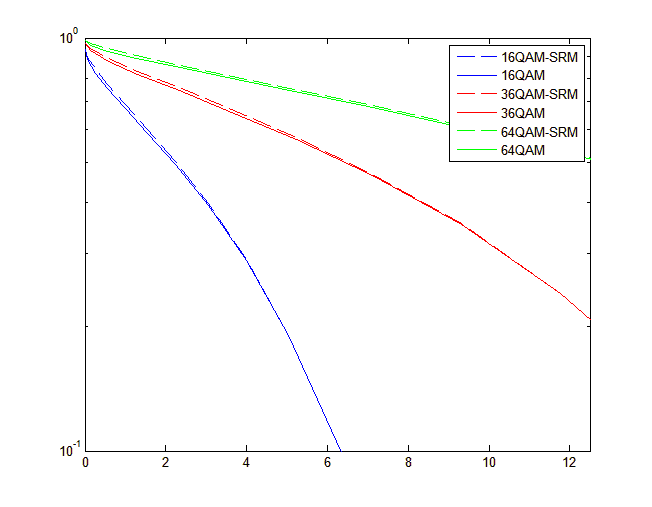
\includegraphics[width=0.5\textwidth]{figures/chap2/SRM-vs-Helstrom}
  \caption{QAM信号平方根检测与Helstrom极限}
  \label{fig:SRM-vs-Hel}
\end{figure}


\section{现有的量子接收机简介}

\subsection{二进制信号量子接收机}




\subsection{PSK信号量子接收机}





\subsection{其它类型量子接收机}






\section{量子信道编码理论}

\subsection{Holevo容量}






\subsection{常见的量子编码方案}





